\documentclass[25pt,landscape]{tikzposter}
\usepackage[utf8]{inputenc}
\usepackage{multicol}
\usepackage{xcolor}
\usepackage{blindtext}
\usepackage{comment}

\title{Clasificación de Textos: Naive Bayes vs Neural Networks}
\author{David Pérez Gómez \& Guzmán López Santamaría}
\date{}
\institute{EUITI - UPV/EHU}

\usetheme{Simple}
\usecolorstyle{Denmark}

\tikzposterlatexaffectionproofoff

\settitle{ \centering \vbox{
\centering
\color{white} {\bfseries \Huge \sc \@title \par}
\vspace*{1em}
{\huge \@author \par} \vspace*{1em} {\LARGE \@institute}
}}


\begin{document}

\maketitle
\begin{columns}
	\column{0.30}
	\block{Objetivos}{
	Dado un conjunto de datos de autopsias verbales se quiere realizar un proceso de clasificación mediante el cual se prediga una clase para cada instancia. Este proceso se llevará a cabo mediante dos clasificadores diferentes y representando el conjunto de datos de dos formas distintas. El objetivo de este proyecto es analizar y comparar los resultados obtenidos para cada uno de los clasificadores y de las representaciones.
	}

	\column{0.40}
	\block{}{
	AQUÍ IRIA UNA PUTA TABLA
	}
	
	\column{0.30}
	\block{Datos}{
	El conjunto de datos es Verbal Autopsies, un conjunto de autopsias verbales realizadas en diversos países y que agrupa una gran variedad de enfermedades y causas de muerte. Serán estas las que nuestro clasificador utilice como clase a predecir.
	En cuanto a las entradas, utilizaremos el atributo correspondiente a la autopsia verbal en sí (gs\_text34). 
	}	
	
\end{columns}	

\begin{columns}
	\column{0.30}
	\block{Representación de Textos}{}
    \block{TF-IDF}{
		TF-IDF es una medida estadística que sirve para calcular la importancia de una palabra dentro de un texto. De forma simplificada, se considera que la importancia de una palabra aumenta cuantas más apariciones tenga en un documento dado, pero a su vez es inversamente proporcional a su ratio de aparición en otros documentos.
    }
    \block{Document Embeddings}{
		Explicación.
		
		Gensim.
    }
    \column{0.30}
   	\block{Clasificadores}{}
	\block{Naive Bayes}{
		\paragraph{}Como clasificador de referencia hemos decidido utilizar Naive Bayes. Este algoritmo calcula la probabilidad de pertenencia a cada clase para cada atributo en función de su valor. Con esto se está suponiendo que los atributos son independientes entre sí. Cuando se dispone a clasificar, realiza la predicción en función de las probabilidades calculadas para cada uno de los atributos de la instancia dada y selecciona la clase que maximice esta probabilidad.
		\paragraph{}Debido a que Naive Bayes asume una total independencia entre clases, consideramos que este clasificador es una buena base para comparar con otro clasificador más complejo.
    }
    \block{Redes Neuronales}{
		\blindtext
    }

    \column{0.40}
    \block{Resultados}{
		\blindtext
		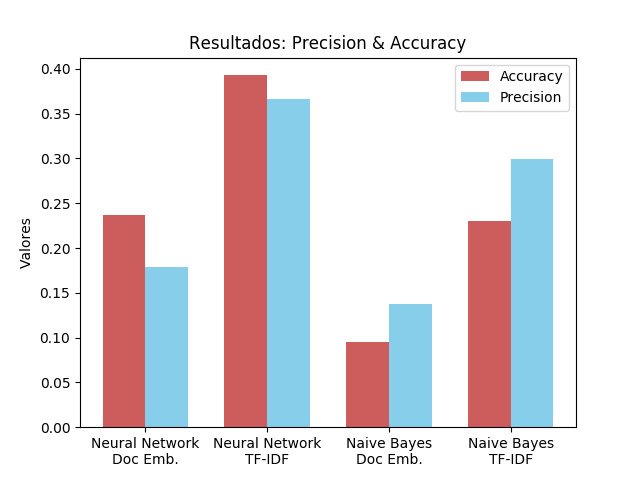
\includegraphics[scale=2]{img/PrecisionAccuracy.jpeg}
    }
    
\end{columns}
 	
\end{document}